\section{Introducción}
\bigskip

El presente informe detalla el diseño e implementación de un amplificador de audio clase G. En la realización de este proyecto han sido volcados los conocimientos de la materia Circuitos Electrónicos II. En la Figura~\ref{esquema_bloques}, se muestra el diagrama en bloques de las partes fundamentaes del proyecto.
	
	\begin{figure}[H]
	\centering
	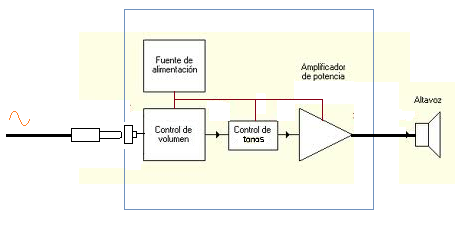
\includegraphics[scale=0.65]{img/esquema_bloques.png}
	\caption{Esquema en bloques.}
	\label{esquema_bloques} 
	\end{figure}
	
	
Un preamplificador es un circuito que permite adaptar las diferentes señales de entrada para luego poder ingresarlas a una etapa de potencia. Este circuito puede servir para adaptar señales de diferentes fuentes, por ejemplo: micrófonos, reproductores de mp3, salidas de placas de sonido de  pc, etc. Como todos estos dispositivos no tienen el mismo nivel de salida, el preamplificador es quien se encarga de llevar a todas estas señales a una tensión de estipulada que luego entra a la etapa de potencia anteriormente nombrada. Los preamplificadores suelen ser de baja potencia y de realizarse de forma adecuada no deben distorsionar en gran medida la señal.

Alguno de los controles que pueden tener los preamplificadores son:
	
\begin{itemize}
	\item Control de volumen
	\item Control de tono
	\item Control de balance
	\item Selector de canal de entrada 
	\item Amplificación
	\end{itemize}	
	
Un amplificador debe satisfacer ciertos requerimientos especiales. Uno de los más importantes es el de entregar una señal con una cantidad específica de potencia a una carga con niveles aceptablemente bajos de distorsión. Otro objetivo común en el diseño es minimizar la impedancia de salida, de tal forma que la ganancia de voltaje quede relativamente poco afectada por el valor de la impedancia de carga. Una etapa de salida bien diseñada debe cumplir con estas características de funcionamiento, consumiendo poca potencia en estado de reposo, sin que esto represente una limitación importante en la respuesta en frecuencia del amplificador. 
 

Los amplificadores de potencia  se clasifican generalmente en seis tipos: A, B, AB , C y G para diseños analógicos y clases D y E para los diseños de conmutación. 
\medskip 
\subsubsection*{Amplificadores clase A.}


En esta clase de amplificadores se usa un solo transistor. El emisor seguidor es la etapa de salida clase A mas utilizada. La corriente de salida circula durante todo el ciclo de la señal de entrada, ya que el transistor esta polarizado con una corriente continua. Esta es una de las grandes desventajas de este tipo de amplificador ya que consume potencia en ausencia de señal y por lo tanto es lógico esperar un rendimiento pobre que en general no supera el 25\%. Como ventaja la distorsión introducida suele ser baja. En la Figura~\ref{ampliA} se muestra un ejemplo de este tipo de amplificador.
 
\begin{figure}[H]
\centering
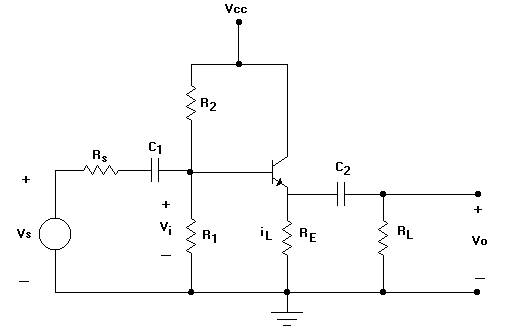
\includegraphics[scale=0.6]{img/ampliA.png}
\caption{Ejemplo, amplificador clase A}
\label{ampliA} 
\end{figure}

\medskip 
\subsubsection*{Amplificador clase B}

Esta clase de amplificadores se compone de un par de transistores (uno pnp y otro npn) conectados de forma tal que no se encuentren ambos en la zona de modo activo directo en el mismo instante de tiempo. Es decir, si suponemos tener una entrada senoidal, durante un semiciclo uno de los transistores se encuentra en la región activa, conduciendo corriente, mientras que el otro se encuentra en corte y durante el otro semiciclo viceversa.
 Una ventaja de esta amplificador sobre la clase A, es que los transistores no disipan potencia en ausencia de señal, lo cual mejora la vida util de los transistores y el rendimiento notablemente, alcanzando un máximo del 78\%.
 La desventaja en este tipo de amplificadores es la llamada “distorsión por cruce”. Es fácil detectar su procedencia al analizar la Figura~\ref{ampliB}.

\begin{figure}[H]
\centering
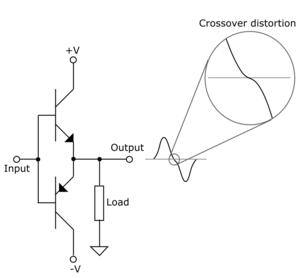
\includegraphics[scale=0.8]{img/ampliB.png}
\caption{Ejemplo, salida clase B.}
\label{ampliB} 
\end{figure}


Se observa que hay un intervalo de tensiones en el cual los transistores no conducen, ese rango generalmente esta dado por $\pm$0.7 V y esta dado por las curvas características de transferencia.

\medskip 
\subsubsection*{Amplificador clase “AB”}


 Este tipo de amplificadores recurre a la misma topología utilizada en la etapa de salida de los amplificadores clase B, con la salvedad de que aquí en los transistores circulan una corriente de polarización a modo de reducir notablemente la “distorsión por cruce”.
 Existen diferentes formas de logra dicho tipo de polarización. Las mas sencillas implican agregar un resistor o diodos, por los que circula una corriente fija dada por el circuito de polarización o fuente de corriente. La otra forma es utilizar los circuitos conocidos como multiplicadores de VBE , que resulta ser la forma empleada en este trabajo práctico.

\medskip 
\subsubsection*{Amplificador clase C}


La corriente de salida solo circula durante menos de medio ciclo de la señal de entrada. Y luego se complementa la salida con un circuito compuesto de capacitores e inductores.
La clase C trabaja para una banda de frecuencias estrecha y resulta muy apropiado en equipos de radiofrecuencia. Esto es debido al fenómeno de resonancia el cual se genera a la salida del amplificador cuando es sintonizado (la impedancia capacitiva e inductiva se cancelan a una frecuencia previamente calculada), aunque no trabaja arriba de 180 grados de ciclo, este amplificador a la salida genera una señal de ciclo completo de señal para la frecuencia fundamental. En la Figura~\ref{ampliC} se muestra un ejemplo de una amplificador de esta clase.
No se utiliza en sonido, por su gran nivel de distorsión y por que su operación no esta destinada para amplificadores de gran señal o gran potencia.

\begin{figure}[H]
\centering
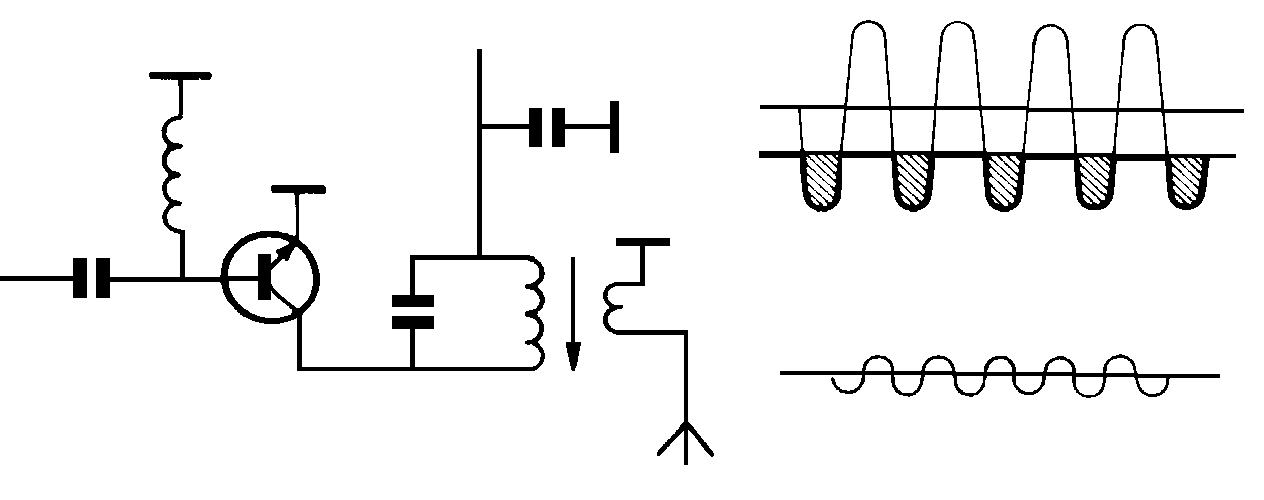
\includegraphics[scale=0.35]{img/ampliC.png}
\caption{Ejemplo, amplificador clase C.}
\label{ampliC} 
\end{figure}

\medskip 
\subsubsection*{Amplificador clase D}

Esta clase de amplificadores usa señales de pulso (digitales). El uso de técnicas digitales hace posible obtener una señal que varía a lo largo del ciclo completo para producir la salida a partir de muchas partes de la señal de entrada. La principal ventaja de la operación en clase D es que los transistores MOSFET de salida trabajan solo en corte y saturación por lo que teóricamente no se disipa potencia en forma de calor y la eficiencia general puede ser muy alta, de entre 90\% a 99\%. En la practica los MOSFETS solo disipan potencia cuando se encuentran conduciendo (saturación) debido a la pequeña resistencia de encendido que poseen, llamada $R_dson$, de todas maneras esta potencia es despreciable ya que $R_dson$ es del orden de las milésimas de ohm. Se utilizan transistores MOSFET ya que son los únicos capaces de conmutar a las elevadas frecuencias de trabajo, del orden de las centenas de KHz llegando a los MHz en algunos casos.


%El desarrollo del trabajo fue encarado como un caso real de la vida profesional, en el cual se nos han dado las especificaciones y basamos en ellas nuestro diseño, tratando de ser lo mas eficientes al menor costo posible y con los productos que se pudieron encontrar en el mercado.
%	
%Durante el desarrollo del trabajo hemos ido encontrando inconvenientes, ya sea errores humanos o diferencias entre las simulaciones y la implementación material. Se detallaron dichos problemas ya que consideramos que contribuyen al proceso de aprendizaje del diseño real.